\chapter{Démonstrateur}

Une fois la carte électronique développée, il était nécessaire de déterminer un \textit{use case} pouvant être utilisé comme démonstrateur complet du travail réalisé. En somme, la création d'un capteur générique qui puisse fournir tous les types de données générées. Le but était d'utiliser l'intégralité de l'infrastructure mise à disposition, en partant du \textit{périphérique} (SmartCanton DevBox dans ce cas) jusqu'à la visualisation des données à l'aide d'une interface, en passant par l'approvisionnement de l'AppKey LoRaWAN.


\section{Architecture finale}

\begin{figure}[ht!]
    \centering
    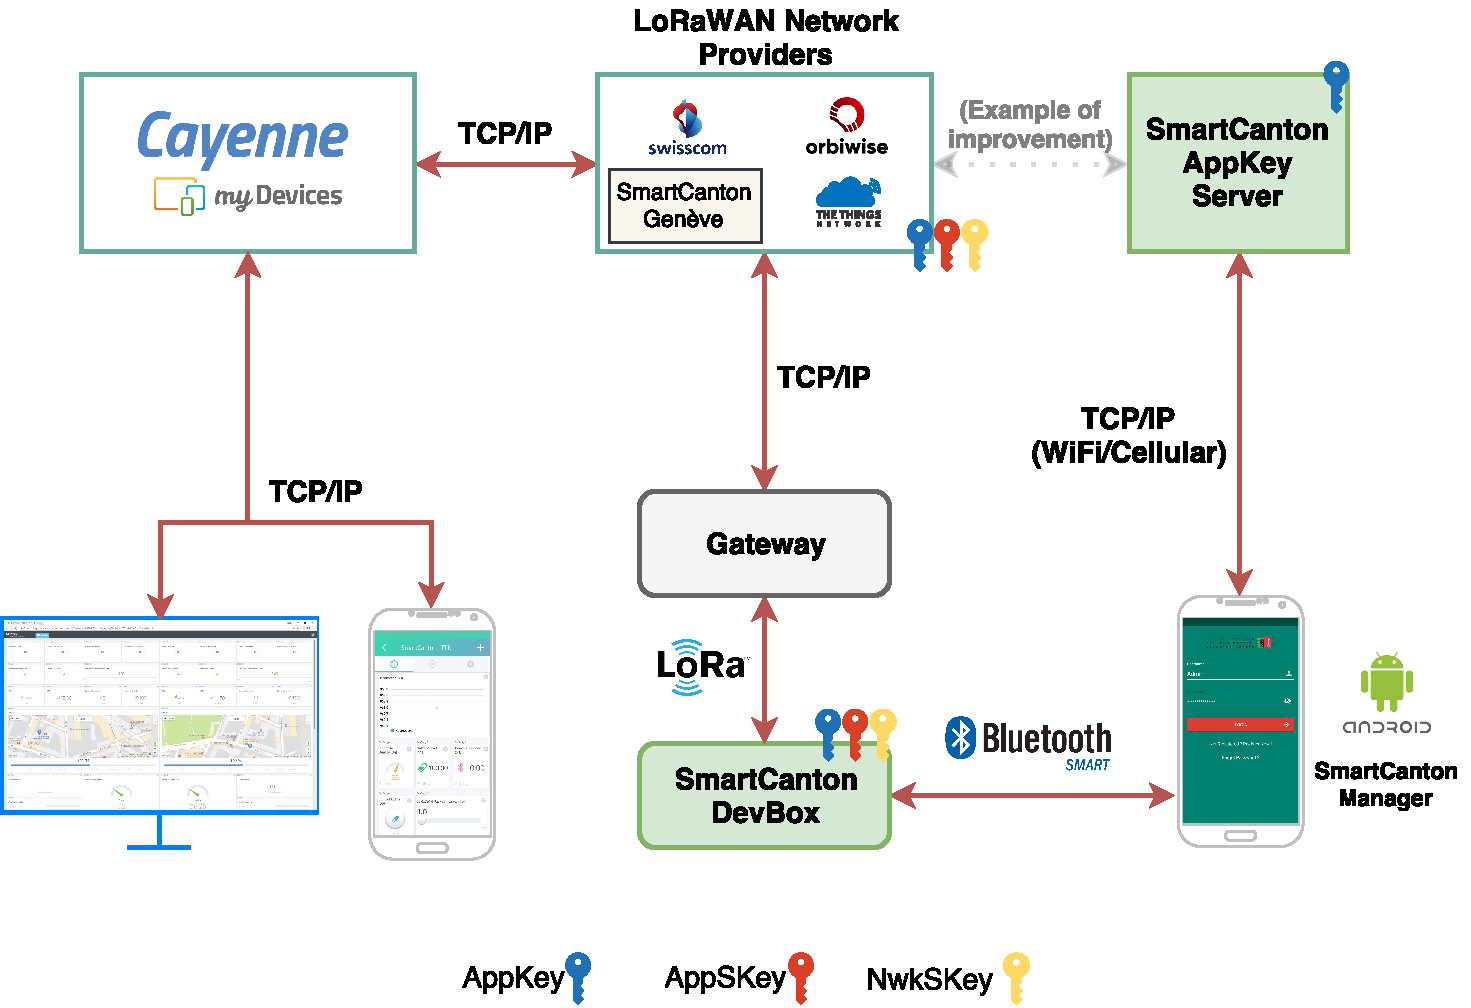
\includegraphics[width=1.0\textwidth]{Figures/Software/smartcanton_overall_project_view.pdf}
    \caption{Diagramme du projet avec l'application de visualisation des données}
    \label{fig-smartcanton_overall_project_view}
\end{figure}

La plateforme Cayenne de l'entreprise MyDevice a été raccordée au flux de données proposé par les différents opérateurs LoRaWAN. Ce démonstrateur permet d'utiliser tous les périphériques disponibles sur la carte électronique développée et de les visualiser sur des terminaux. Les données sont toutes accessibles via \textit{Bluetooth Low Energy} ou \textbf{LoRaWAN}. Le débit des données par LoRaWAN a été limité à maximum un paquet par seconde, et ceci en désactivant le contrôle du \textit{duty cycle} de la \textit{stack} LoRaWAN.

\section{Cayenne de MyDevices}

Cayenne est une plateforme qui offre la possibilité d'afficher des \textit{widgets} contenant diverses données prodiguées par l'utilisateur. L'utilisateur peut choisir plusieurs formats d'affichage pour les données (ex. valeur instantanée, graphique, jauge, etc.). Des actuateurs peuvent également être intégrés afin de générer des données ou des événements en direction du périphérique. \\

Le support des périphériques LoRa est encore en bêta sur la plateforme, mais beaucoup d'opérateurs sont déjà supportés pour la récupération des données. Parmi ces opérateurs LoRaWAN, on identifie la présence de Swisscom, Orbiwise et The Things Network, tous actifs dans la région genevoise. The Things Network dispose d'un très bon tutoriel\footnote{\url{https://www.thethingsnetwork.org/docs/devices/arduino/api/cayennelpp.html}} pour l'intégration avec Cayenne. C'est d'ailleurs par ce biais que la plateforme a été découverte.

\subsection{Format des données}
Dans la tâche RTOS DevBox Main, il était nécessaire de respecter le format de données imposé par Cayenne, de sorte que celles-ci soient interprétées par la plateforme. La description complète des commandes, de même que des exemples de trames sont disponibles dans la documentation de Cayenne : 
\begin{center}
    \url{https://mydevices.com/cayenne/docs/lora/}
\end{center}

Bien que le format des données ne soit nullement optimisé pour une application prévue en production, il est nécessaire pour que Cayenne puisse interpréter correctement ces dernières. Une bibliothèque C++ a été adaptée en C afin que la conversion des données soit simplifiée. La bibliothèque initialement utilisée est disponible à l'adresse suivante : 
\begin{center}
    \url{https://github.com/sabas1080/CayenneLPP}
\end{center}


\subsection{Fonctionnalités implémentées}

Toutes les données des capteurs sont envoyées à l'aide de paquets \textit{uplinks}. Voici la liste de celles-ci :
\begin{enumerate}
    \item RSSI;
    \item SNR;
    \item latitude et longitude GPS;
    \item BNO055 (accéléromètre et gyroscope);
    \item BME680 (température, humidité, pression et IAQ);
    \item \textit{beacons} Bluetooth Low Energy scannés;
    \item niveau de batterie.\\
\end{enumerate}

Des actuateurs sont disponibles sur les \textit{dashboards} pour générer des messages \textit{downlinks} LoRaWAN. L'état de ces actuateurs est également envoyé dans les paquets \textit{uplink}, afin que l'affichage soit toujours à jour. En voici l'énumération :
\begin{enumerate}
    \item autoriser l'envoi des données du GPS;
    \item autoriser l'envoi des données du BNO055 (accéléromètre + gyroscope);
    \item autoriser l'envoi des données du BME680 (température, humidité, pression et IAQ);
    \item autoriser l'envoi des données du niveau de batterie;
    \item autoriser l'envoi des données du scanneur de \textit{beacons} BLE;
    \item intervalle entre chaque paquet LoRaWAN configurable en secondes;
    \item contrôle de l'état de la LED verte connectée au KW41Z.\\
\end{enumerate}

Dans l'état actuel du démonstrateur, ces configurations ne sont pas sauvegardées dans la mémoire non volatile du KW41Z. Lors du \textit{reset} de celui-ci, une configuration préprogrammée est appliquée. Par défaut, toutes les autorisations d'envoi des mesures sont activées et l'intervalle entre chaque paquet est de 4min. La LED verte est quant à elle éteinte.

\subsection{Dashboard}

Le dashboard est visualisable en ligne dans un navigateur Web. Le dashboard est personnalisable par le développeur et peut ensuite être partagé avec un lien. Lors de ce partage, des droits d'accès peuvent être spécifiés, tels que l'activation des actuateurs. Un exemple de dashboard affichant les données d'une DevBox est présenté sur la \cref{fig-cayenne_dashboard_allsensors}.
Cayenne propose également la possibilité de visualiser les diverses informations des capteurs à l'aide d'une application Android\footnote{\url{https://play.google.com/store/apps/details?id=com.mydevices.cayenne}}, visible sur la \cref{fig-cayenne_dashboard_allsensors_android}. Celle-ci est toute fois un peu instable selon les menus sélectionnés.

\begin{figure}[ht!]
    \centering
    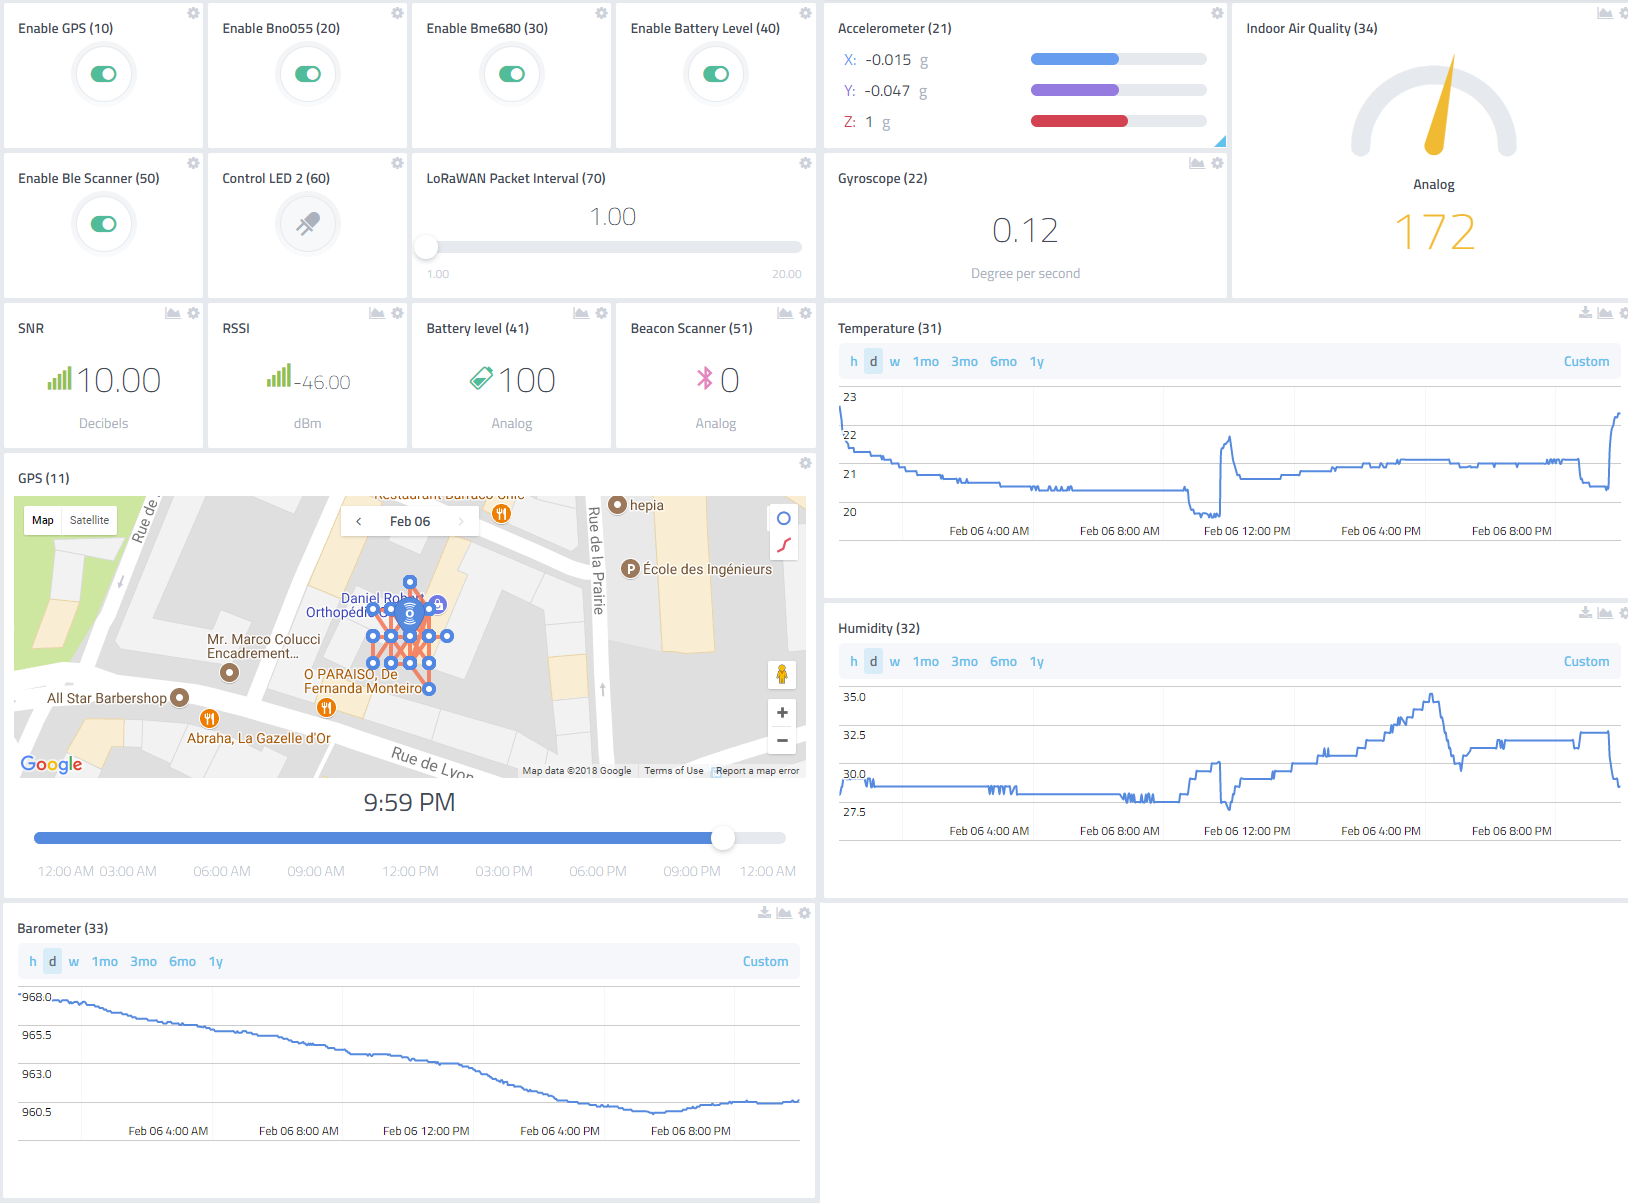
\includegraphics[width=1.0\textwidth]{Figures/UseCase/cayenne_dashboard_allsensors.png}
    \caption{\textit{Dashboard} du capteur DevBox à l'aide de Cayenne sur un navigateur Web}
    \label{fig-cayenne_dashboard_allsensors}
\end{figure}


\begin{figure}[ht!]
    \centering
    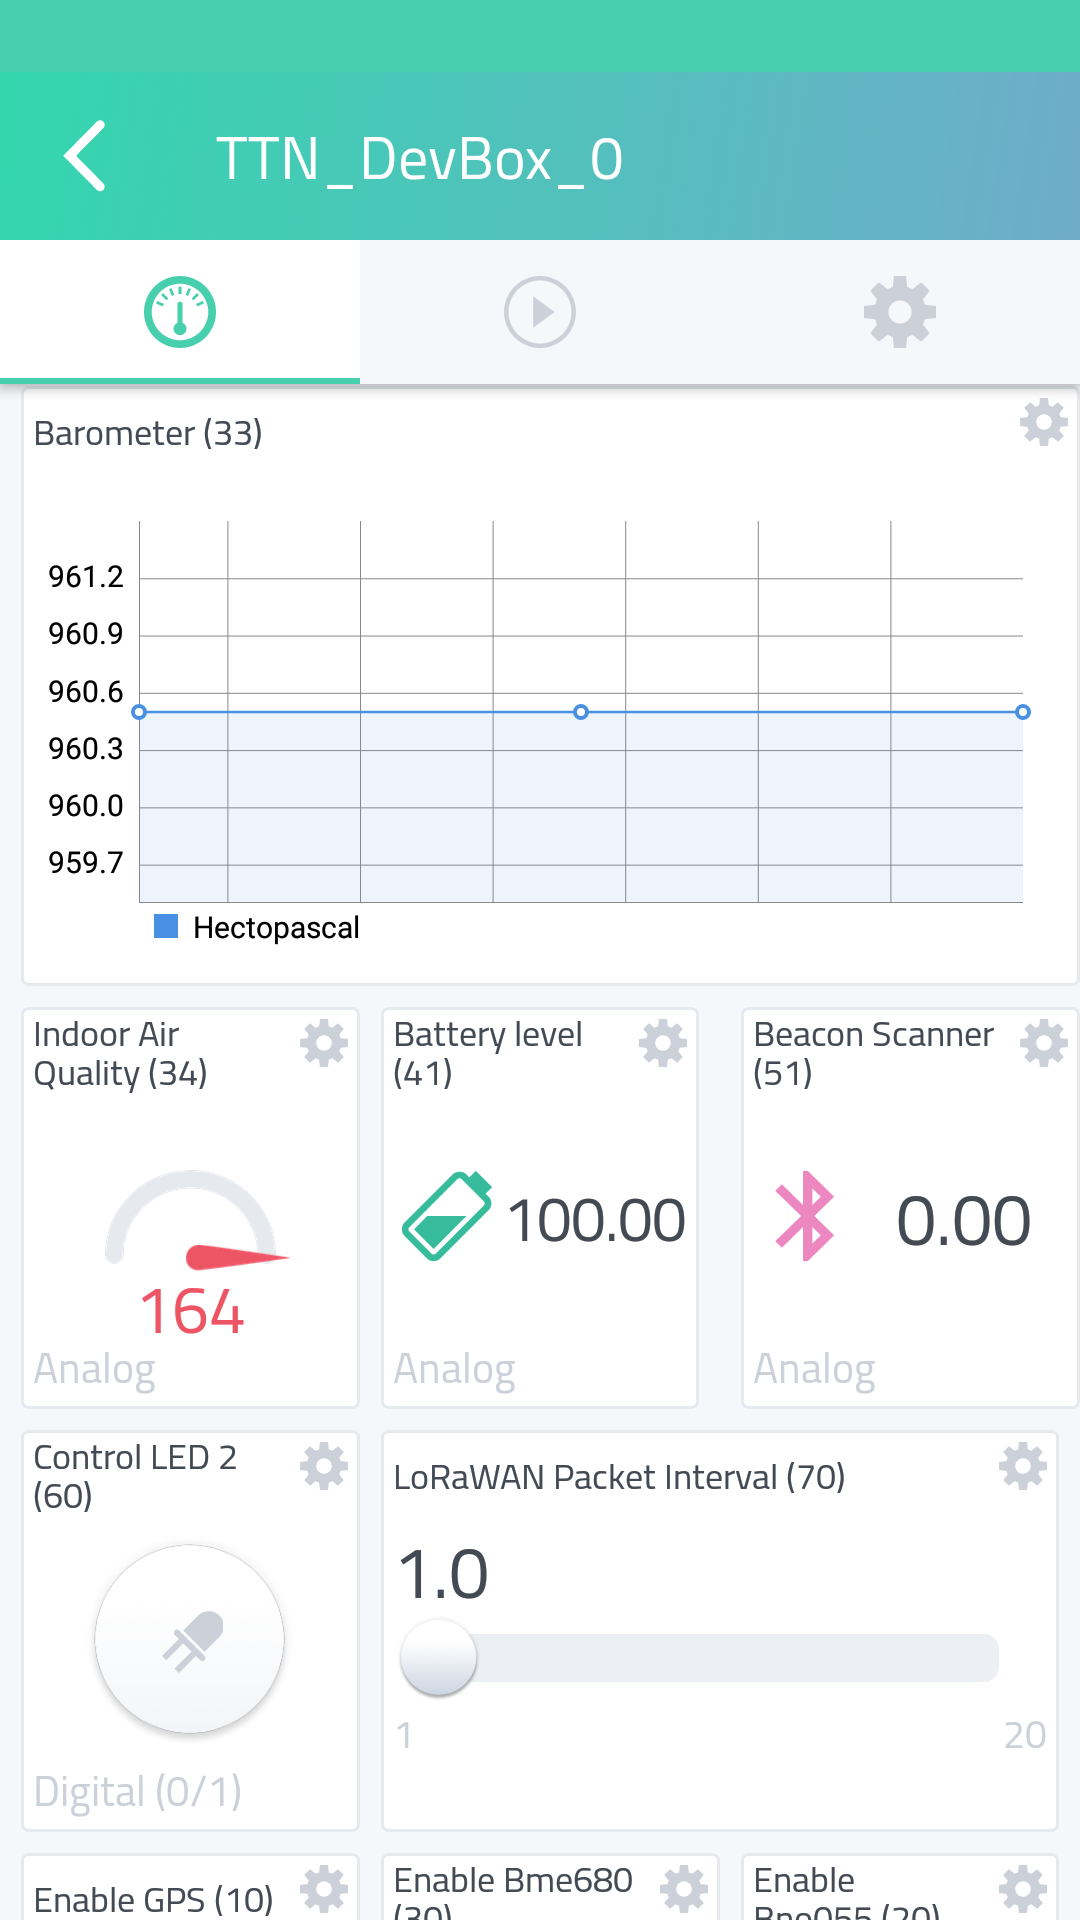
\includegraphics[width=0.3\textwidth]{Figures/UseCase/cayenne_dashboard_allsensors_android.png}
    \caption{\textit{Dashboard} du capteur DevBox à l'aide de Cayenne sur l'application Android}
    \label{fig-cayenne_dashboard_allsensors_android}
\end{figure}


\section{Échangeur d'AppKey}


L'application SmartCanton Manager offre la possibilité de mettre à jour l'AppKey et l'App EUI présents sur la DevBox. Les images démontrant le fonctionnement de l'application ainsi que les étapes de mise à jour sont décrites dans l'\cref{AppendixAndroidAppUserGuide} de ce document. \\

Le serveur est hébergé à hepia à l'aide d'une adresse IP publique fixe. Actuellement, l'AppKey doit être provisionnée à la main dans la base de données SQLite. À l'avenir, la solution de connecter le serveur au HSM ou à une API intermédiaire serait optimale.


\section{Opérateurs testés}

L'application finale a été utilisée principalement sur deux opérateurs: The Things Network (TTN) et Orbiwise. La plus grande partie du développement a été réalisée sur TTN, plusieurs \textit{gateways} LoRaWAN étant disponibles dans les locaux d'hepia. Cayenne supporte les deux opérateurs pour recevoir des données sur les \textit{dashboards}. Il est ainsi aisé d'alterner les réseaux à l'aide de l'application SmartCanton Manager et de visualiser le changement du flux de données entre les deux \textit{dashboards} (TTN et Orbiwise). Toutefois, les \textit{downlinks} sur Orbiwise ne semblent pas être correctement supportés par la plateforme Cayenne pour l'instant.

\section{Consommation électrique}

La consommation électrique du périphérique n'a malheureusement pas pu être optimisée pour le démonstrateur final. C'est un choix qui s'est imposé lors du développement pour accélérer la réalisation d'un prototype fonctionnel. Lors de la réalisation du PCB, quelques erreurs ont naturellement été commises, ce qui a provoqué des problèmes de consommation (ex. la connexion de l'antenne LoRa, cf. \cref{sec_hardware_errors}).

Le circuit présente actuellement une consommation moyenne de 100\,mA. La source de 50\,\% de cette consommation est connue et émane du GPS. En effet, avec son antenne active, le GPS consomme environ 50\,mA (cf. \cref{sec-hardware_gps}). Le reste de la consommation provient des divers périphériques, tels que les LEDs qui utilisent chacune 4 à 6\,mA. Le processeur n'a pas été mis en mode \textit{low power}. Ce mode est actionnable à l'aide d'une \textit{macro} dans le SDK. Pour des raisons de temps, ce mode n'a toutefois pas pu être testé en vue d'examiner sa stabilité. 



